\section*{algorithmic techniques: linear programming (rounding)}
\addcontentsline{toc}{section}{algorithmic techniques: linear programming (rounding)}

% $$$$$$$$$$$$$$$$$$$$$$$$$$$$$$$$$$$$$$$$$$$$$$$$$$$$$$$$$$$$$$$$$$$$$$$$$$$$$$$$

\subsection*{caratteristiche}
\addcontentsline{toc}{subsection}{caratteristiche}
\begin{flushleft}
	\begin{itemize}
		\item il problema \'e formulato come un programma lineare intero (ILP: integer linear program)
		\item programma lineare intero: programmi lineare + vincoli di interezza
		\item esiste un algoritmo con complessit\'a temporale polinomale (algoritmo ellissoide) per risolvere problemi lineari, ma...
		\item risolvere un programma lineare intero \'e un problema NP-HARD
		\item la formulazione come ILP consente di utilizzare potenti mezzi generali che, in base alle propriet\'a dell'ILP, sono in grado di fornire algoritmi con buona approssimazione:
		\begin{itemize}
			\item rounding (arrotondamento)
			\item primal-dual (primale-duale)
		\end{itemize}
	\end{itemize}
\end{flushleft}

% $$$$$$$$$$$$$$$$$$$$$$$$$$$$$$$$$$$$$$$$$$$$$$$$$$$$$$$$$$$$$$$$$$$$$$$$$$$$$$$$

\subsection*{rounding: caratteristiche}
\addcontentsline{toc}{subsection}{rounding: caratteristiche}
\begin{flushleft}
	\begin{itemize}
		\item il problema \'e formulato come un programma lineare
		\item il rilassamento lineare (LP) viene ottenuto dall'ILP rilassando i vincoli d'interezza, ovvero sostituendoli con adeguati vincoli lineari (sugli interi)
		\item la soluzione ottenuta (ottima per LP) \'e arrotondata ad una vicina soluzione intera ammissibile per ILP
		\item la misura $m$ della soluzione ottenuta \'e in seguito confrontata con quella della soluzione ottima LP, ovvero $m_{LP}^*$, cio\'e un limite inferiore ($\min$) o superiore ($\max$) per $m^*$
	\end{itemize}
	\vspace{0.5cm}
	\begin{center}
		\textbf{min problems}\newline \\
		\vspace{0.3cm}
		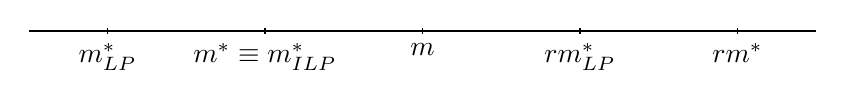
\begin{tikzpicture}
			\draw[thick,-] (0,0) -- (10,0);
			\draw(1,1pt) -- (1,-1pt) node[anchor=north] {$m_{LP}^*$};
			\draw(3,1pt) -- (3,-1pt) node[anchor=north] {$m^*\equiv m_{ILP}^*$};
			\draw(5,1pt) -- (5,-1pt) node[anchor=north] {$m$};
			\draw(7,1pt) -- (7,-1pt) node[anchor=north] {$rm_{LP}^*$};
			\draw(9,1pt) -- (9,-1pt) node[anchor=north] {$rm^*$};
		\end{tikzpicture}
	\end{center}
	\begin{center}
		\textbf{max problems}\newline \\
		\vspace{0.3cm}
		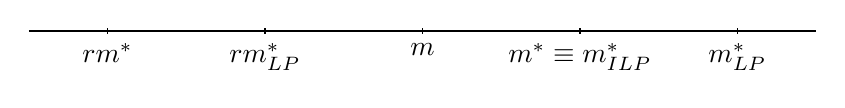
\begin{tikzpicture}
			\draw[thick,-] (0,0) -- (10,0);
			\draw(1,1pt) -- (1,-1pt) node[anchor=north] {$rm^*$};
			\draw(3,1pt) -- (3,-1pt) node[anchor=north] {$rm_{LP}^*$};
			\draw(5,1pt) -- (5,-1pt) node[anchor=north] {$m$};
			\draw(7,1pt) -- (7,-1pt) node[anchor=north] {$m^*\equiv m_{ILP}^*$};
			\draw(9,1pt) -- (9,-1pt) node[anchor=north] {$m_{LP}^*$};
		\end{tikzpicture}
	\end{center}
\end{flushleft}

% $$$$$$$$$$$$$$$$$$$$$$$$$$$$$$$$$$$$$$$$$$$$$$$$$$$$$$$$$$$$$$$$$$$$$$$$$$$$$$$$

\subsection*{problema: min weighted vertex cover}
\addcontentsline{toc}{subsection}{problema: min weighted vertex cover}
\begin{flushleft}
	\begin{itemize}
		\item INPUT:
		\begin{itemize}
			\item un grafo $G=(V,E)$
			\item un costo intero $c_j$ associato ad ogni $v_j\in V$
		\end{itemize}
		\item SOLUZIONE:
			$$U\subseteq V\text{ }\vert\text{ }v_j\in U\vee v_k\in U\text{, }\forall\{v_j,v_k\}\in E$$
		\item MISURA: costo totale di U, ovvero
			$$\sum_{v_j\in U}c_j$$
	\end{itemize}
\end{flushleft}

% $$$$$$$$$$$$$$$$$$$$$$$$$$$$$$$$$$$$$$$$$$$$$$$$$$$$$$$$$$$$$$$$$$$$$$$$$$$$$$$$

\subsection*{ILP: min weighted vertex cover}
\addcontentsline{toc}{subsection}{ILP: min weighted vertex cover}
\begin{flushleft}
	\begin{itemize}
		\item funzione obiettivo: $\min\sum_{j=1}^n c_jx_j$
		\item vincoli: $x_j+x_k\geq 1\text{, }\forall\{v_j,v_k\}\in E$
		\item vincoli interi: $x_j\in\{0,1\}\text{, }\forall v_j\in V\text{, }\forall j\text{ con }1\leq j\leq n$
	\end{itemize}
\end{flushleft}

% $$$$$$$$$$$$$$$$$$$$$$$$$$$$$$$$$$$$$$$$$$$$$$$$$$$$$$$$$$$$$$$$$$$$$$$$$$$$$$$$

\subsection*{LP: min weighted vertex cover (rilassamento lineare)}
\addcontentsline{toc}{subsection}{LP: min weighted vertex cover (rilassamento lineare)}
\begin{flushleft}
	\begin{itemize}
		\item $\min\sum_{j=1}^n c_jx_j$
		\item $x_j+x_k\geq 1\text{, }\forall\{v_j,v_k\}\in E$
		\item \sout{$x_j\leq 1\text{, }\forall v_j\in V$} (superfluo)
		\item $x_j\geq 0\text{, }\forall v_j\in V$
	\end{itemize}
\end{flushleft}

% $$$$$$$$$$$$$$$$$$$$$$$$$$$$$$$$$$$$$$$$$$$$$$$$$$$$$$$$$$$$$$$$$$$$$$$$$$$$$$$$

\subsection*{algoritmo: Round-Vertex-Cover}
\addcontentsline{toc}{subsection}{algoritmo: Round-Vertex-Cover}
\begin{flushleft}
	\begin{algorithm}
		\caption{Round-Vertex-Cover}
		\begin{algorithmic}
			\STATE determina l'ILP associato all'istanza in input
			\STATE risolvi il rilassamento lineare LP dell'ILP
			\STATE sia $<x_1^*,x_2^*,\ldots,x_n^*>$ la risultante soluzione ottima dell'LP
			\STATE $\forall v_j$ sia $x_j=1$ se $x_j^*\geq\frac{1}{2}$ e $x_j=0$ se $x_j^*<\frac{1}{2}$
			\RETURN il cover $U$ associato a $<x_1^*,x_2^*,\ldots,x_n^*>$, ovvero tale che $U=\{v_j\in V\text{ }\vert\text{ }x_j=1\}$
		\end{algorithmic}
	\end{algorithm}
\end{flushleft}

% $$$$$$$$$$$$$$$$$$$$$$$$$$$$$$$$$$$$$$$$$$$$$$$$$$$$$$$$$$$$$$$$$$$$$$$$$$$$$$$$

\subsection*{teorema: l'algoritmo Round-Vertex-Cover \'e $2$-approssimante}
\addcontentsline{toc}{subsection}{teorema: l'algoritmo Round-Vertex-Cover \'e $2$-approssimante}
\begin{flushleft}
	l'algoritmo Round-Vertex-Cover \'e $2$-approssimante \newline \\
	\textbf{dimostrazione:}
	\begin{itemize}
		\item \'e sufficiente mostrare che:
		\begin{enumerate}
			\item $x_1,x_2,\ldots,x_n$ \'e ammissibile per l'ILP (esso soddisfa tutti i vincoli), ovvero $U$ \'e un cover
			\item $\frac{m}{m_{LP}^*}\leq 2$ e quindi anche $\frac{m}{m^*}\leq\frac{m}{m_{LP}^*}\leq 2$
		\end{enumerate}
		\item DIMOSTRIAMO 1.
		\begin{itemize}
			\item dall'ammissibilit\'a di $<x_1^*,x_2^*,\ldots,x_n^*>$ per LP, per ogni arco $\{v_j,v_k\}\in E$ vale $x_j^*+x_k^*\geq 1$
			\item ovvero $x_j^*\geq 0.5$ o $x_k^*\geq 0.5$, cos\'i che $x_j=1$ o $x_k=1$, e quindi $x_j+x_k\geq 1$ \'e soddisfatto in ILP
		\end{itemize}
		\hfill$\blacksquare$
		\item DIMOSTRIAMO 2.
		\begin{itemize}
			\item[] $$m=\color{gray}\sum_{j=1}^nc_jx_j\ldots$$
			\item (dall'arrotondamento: $x_j\leq 2x_j^*$)
			\item[] $$m=\sum_{j=1}^nc_jx_j\leq\sum_{j=1}^nc_j2x_j^*=2\color{gray}\sum_{j=1}^nc_jx_j^*\ldots$$
			\item ($\sum_{j=1}^nc_jx_j^*=m_{LP}^*$)
			\item[] $$m=\sum_{j=1}^nc_jx_j\leq\sum_{j=1}^nc_j2x_j^*=2\sum_{j=1}^nc_jx_j^*=2m_{LP}^*$$
			\item ovvero:
				$$\frac{m}{m^*}\leq\frac{m}{m_{LP}^*}\leq 2$$
		\end{itemize}
		\hfill$\blacksquare$
	\end{itemize}
	\hfill$\square$
\end{flushleft}

% $$$$$$$$$$$$$$$$$$$$$$$$$$$$$$$$$$$$$$$$$$$$$$$$$$$$$$$$$$$$$$$$$$$$$$$$$$$$$$$$

\subsection*{problema: min weighted set cover}
\addcontentsline{toc}{subsection}{problema: min weighted set cover}
\begin{flushleft}
	\begin{itemize}
		\item INPUT:
		\begin{itemize}
			\item un universo $U=\{o_1,o_2,\ldots,o_n\}$ di $n$ oggetti
			\item una famiglia $\hat{S}=\{S_1,S_2,\ldots,S_h\}$ di $h$ sottoinsiemi di $U$
			\item un costo intero $c_j$ associato ad ogni $S_j\in \hat{S}$
		\end{itemize}
		\item SOLUZIONE: un cover di $U$, ovvero una sottofamiglia $\hat{C}\subseteq\hat{S}$ tale che:
			$$\cup_{S_j\in\hat{C}}S_j=U$$
		\item MISURA: costo totale del cover, ovvero
			$$\sum_{S_j\in\hat{C}}c_j$$
	\end{itemize}
	\vspace{0.5cm}
	\begin{itemize}
		\item $f=$ frequenza massima di un oggetto nel sottoinsieme $\hat{S}$, ovvero ciasun oggetto occorre in al massimo $f$ sottoinsiemi
		\item dato un insieme di $n$ elementi $\{1,2,\ldots,n\}$ (chiamato universo) e una collezione $S$ di $m$ insiemi, la cui unione eguaglia l'universo, il problema del set cover consiste nell'identificare il pi\'u piccolo sottoinsieme di $S$ la cui unione eguaglia l'universo
	\end{itemize}
\end{flushleft}

% $$$$$$$$$$$$$$$$$$$$$$$$$$$$$$$$$$$$$$$$$$$$$$$$$$$$$$$$$$$$$$$$$$$$$$$$$$$$$$$$

\subsection*{ILP: min weighted set cover}
\addcontentsline{toc}{subsection}{ILP: min weighted set cover}
\begin{flushleft}
	\begin{itemize}
		\item funzione obiettivo: $\min\sum_{j=1}^h c_jx_j$
		\item vincoli: $\sum_{S_j\vert o_i\in S_j}x_j\geq 1\text{, }\forall o_i\in U$
		\item vincoli interi: $x_j\in\{0,1\}\text{, }\forall S_j\in\hat{S}$
	\end{itemize}
\end{flushleft}

% $$$$$$$$$$$$$$$$$$$$$$$$$$$$$$$$$$$$$$$$$$$$$$$$$$$$$$$$$$$$$$$$$$$$$$$$$$$$$$$$

\subsection*{LP: min weighted set cover (rilassamento lineare)}
\addcontentsline{toc}{subsection}{LP: min weighted set cover (rilassamento lineare)}
\begin{flushleft}
	\begin{itemize}
		\item $\min\sum_{j=1}^h c_jx_j$
		\item $\sum_{S_j\vert o_i\in S_j}x_j\geq 1\text{, }\forall o_i\in U$
		\item \sout{$x_j\leq 1\text{, }\forall S_j\in\hat{S}$} (superfluo)
		\item $x_j\geq 0\text{, }\forall S_j\in\hat{S}$
	\end{itemize}
\end{flushleft}

% $$$$$$$$$$$$$$$$$$$$$$$$$$$$$$$$$$$$$$$$$$$$$$$$$$$$$$$$$$$$$$$$$$$$$$$$$$$$$$$$

\newpage
\subsection*{algoritmo: Round-Set-Cover}
\addcontentsline{toc}{subsection}{algoritmo: Round-Set-Cover}
\begin{flushleft}
	\begin{algorithm}
		\caption{Round-Set-Cover}
		\begin{algorithmic}
			\STATE determina l'ILP associato all'istanza in input
			\STATE risolvi il rilassamento lineare LP dell'ILP
			\STATE sia $<x_1^*,x_2^*,\ldots,x_n^*>$ la risultante soluzione ottima dell'LP
			\STATE $\forall S_j$ sia $x_j=1$ se $x_j^*\geq\frac{1}{f}$ e $x_j=0$ se $x_j^*<\frac{1}{f}$
			\RETURN il cover risultante, ovvero $\hat{C}=\{S_j\in\hat{S}\text{ }\vert\text{ }x_j=1\}$
		\end{algorithmic}
	\end{algorithm}
\end{flushleft}

% $$$$$$$$$$$$$$$$$$$$$$$$$$$$$$$$$$$$$$$$$$$$$$$$$$$$$$$$$$$$$$$$$$$$$$$$$$$$$$$$

\subsection*{teorema: l'algoritmo Round-Set-Cover \'e $f$-approssimante ($f\geq 1$)}
\addcontentsline{toc}{subsection}{teorema: l'algoritmo Round-Set-Cover \'e $f$-approssimante ($f\geq 1$)}
\begin{flushleft}
	l'algoritmo Round-Set-Cover \'e $f$-approssimante ($f\geq 1$) \newline \\
	\textbf{dimostrazione:}
	\begin{itemize}
		\item \'e sufficiente mostrare che:
		\begin{enumerate}
			\item $x_1,x_2,\ldots,x_n$ \'e ammissibile per l'ILP
			\item $\frac{m}{m_{LP}^*}\leq f$ e quindi anche $\frac{m}{m^*}\leq\frac{m}{m_{LP}^*}\leq f$
		\end{enumerate}
		\item DIMOSTRIAMO 1.
		\begin{itemize}
			\item dall'ammissibilit\'a di $<x_1^*,x_2^*,\ldots,x_n^*>$ per LP, $\forall o_i\in U$
				$$\sum_{S_j\vert o_i\in S_j}x_j^*\geq 1$$
			\item e poich\'e la somma ha al massimo ($\leq$) $f$ termini, deve esistere $S_j$ contenente $o_i$ tale che $x_j^*\geq\frac{1}{f}$, ovvero tale che $x_j=1$, e quindi:
				$$\sum_{S_j\vert o_i\in S_j}x_j\geq 1$$
		\end{itemize}
		\hfill$\blacksquare$
		\item DIMOSTRIAMO 2.
		\begin{itemize}
			\item[] $$m=\color{gray}\sum_{j=1}^hc_jx_j\ldots$$
			\item (dall'arrotondamento: $x_j\leq fx_j^*$)
			\item[] $$m=\sum_{j=1}^hc_jx_j\leq\sum_{j=1}^hc_jfx_j^*=f\color{gray}\sum_{j=1}^hc_jx_j^*\ldots$$
			\item ($\sum_{j=1}^hc_jx_j^*=m_{LP}^*$)
			\item[] $$m=\sum_{j=1}^hc_jx_j\leq\sum_{j=1}^hc_jfx_j^*=f\sum_{j=1}^hc_jx_j^*=fm_{LP}^*$$
			\item ovvero:
				$$\frac{m}{m^*}\leq\frac{m}{m_{LP}^*}\leq f$$
		\end{itemize}
		\hfill$\blacksquare$
	\end{itemize}
	\hfill$\square$
\end{flushleft}

% $$$$$$$$$$$$$$$$$$$$$$$$$$$$$$$$$$$$$$$$$$$$$$$$$$$$$$$$$$$$$$$$$$$$$$$$$$$$$$$$

\newpage
